\section{Code repository}
All the code for the Laser Learning Environment is publicly available on the repository \url{https://github.com/yamoling/lle}.



\section{Hyperparameters}
\label{apx:hyperparameters}
Hyperparameter search was performed with VDN on a combination of batch sizes (32, 64 and 128 transitions) and memory sizes (50k, 100k and 200k transitions). Then, we have tried training intervals of 1 and 5.

Then, we performed a hyperparameter search for prioritised experience replay on a combination of $\alpha$ (0.3, 0.4, 0.5, 0.6, 0.7, 0.8) and $\beta$ (0.3, 0.4, 0.5, 0.6, 0.7, 0.8).

For random network distillation, we have explored update ratios $p = 0.25, 0.5$ and $1$, then enabled or disabled annealing, and finally tried clipping the intrinsic reward to 1 or to 5.


\begin{table}[h]
    \centering
    \caption{Hyperparameters used across all the experiments}
    \begin{tabular}{l|l|p{7cm}}
        \textbf{Parameter} & \textbf{Value} & \textbf{Comment} \\
        \hline
        Memory size & 50 000 & Transitions\\
        Batch size & 64 & Transitions\\
        Train interval & 5 time steps & \\
        Optimiser & Adam & \\
        $\alpha$ (Learning rate) & 0.0005 & For both $Q$-network and mixer \\
        Grad norm clipping & 10 & Clips both $Q$-network and mixer\\
        $\gamma$ & $0.95$ & Discount factor\\
        $\tau$ & $0.01$ & Soft update rate\\
        $\epsilon_{start}$ & $1$ &\\
        $\epsilon_{min}$ & $0.05$ &\\
        $\epsilon$ annealing & 500k time steps & Linearly annealed\\
        \hline
        $\alpha$ & 0.6 & PER \\
        $\beta$ & 0.5 & PER \\
        $\beta$ annealing & 1m time steps & PER\\
        \hline
        $p$ & $0.25$ & Randomly mask error from RND with probability $p$\\
        IR factor & $2 \rightarrow 0$ & Intrinsic Reward linearly annealed over 1m steps\\
        IR clip & $5$ & IR is clipped to 5 maximum\\
        IR warmup & 64 & The RND is optimised 64 times before issuing any intrinsic reward\\
        \hline
    \end{tabular}
\end{table}

\newpage
\section{Neural network architecture}
\label{apx:nn_architecture}
The $Q$-network is made of two parts with an interconnection: a convolutional neural network of three layers, an interconnect that flattens the CNN, and finally a neural network of three linear layers. This is depicted in \autoref{tab:nn}.

\begin{table}[h]
    \centering
    \caption{$Q$-network architecture}
    \label{tab:nn}
    \begin{tabular}{|llrcr|}
        \hline
         \textbf{Layer type} & \textbf{Activation} & \textbf{Output shape} & \textbf{Stride} & \textbf{Kernel} \\
         \hline
         Input & & $11 \times 13 \times 15$ & &\\
         Conv2D & ReLU & $32 \times 11 \times 13$ & $1$ & $(3 \times 3)$\\
         Conv2D & ReLU & $64 \times 9 \times 11$ & $1$ & $(3 \times 3)$\\
         Conv2D & ReLU & $32 \times 7 \times 9$ & $1$ &  $(3 \times 3)$\\
         Flatten & & $2016$ &&\\
         Concat & & $2020$&&\\
         Linear & ReLU & $64$ &&\\
         Linear & ReLU & $64$ &&\\
         Linear & & $5$ &&\\
         \hline
    \end{tabular}
\end{table}

\section{Results of \textit{n}-steps returns with VDN}
\label{apx:n-step}

\begin{figure}[h]
    \centering
    \begin{tikzpicture}
        \begin{groupplot}[
            group style={group size= 2 by 1},
            height=5cm,
            width=7.4cm, 
            grid=major,
            legend columns=2
            xtick={0, 200000, 400000, 600000, 800000, 1000000},
            xticklabels={0, 0, 200k, 400, 600k, 800k, 1m},
            scaled x ticks=false,
            title style={yshift=-0.2cm},
        ]
            \nextgroupplot[legend to name=luigi, title={Score}, ymin=-1.5, ymax=5.5, xmin=0, xmax=1000000]       
                \plotMean[3-steps]{3step}{score};
                \plotMean[5-steps]{5step}{score};
                \plotMean[7-steps]{7step}{score};
                \plotMean[9-steps]{9step}{score};
            
                \plotCI{3step}{score};
                \plotStd{5step}{score};
                \plotStd{7step}{score};
                \plotStd{9step}{score};

                \coordinate (top-left) at (rel axis cs:0,1);% coordinate at top left of the first plot
                

            \nextgroupplot[title={Exit rate}, ymin=0, ymax=0.25, xmin=0, xmax=1000000]       
                \plotMean{3step}{exit_rate};
                \plotMean{5step}{exit_rate};
                \plotMean{7step}{exit_rate};
                \plotMean{9step}{exit_rate};
            
                \plotCI{3step}{exit_rate};
                \plotStd{5step}{exit_rate};
                \plotStd{7step}{exit_rate};
                \plotStd{9step}{exit_rate};

                \coordinate (top-right) at (rel axis cs:1,1);
        \end{groupplot}
        \path (top-left)--(top-right) coordinate[midway] (h-center);
        \node[above=0.2cm, inner sep=0pt] at (h-center) {\pgfplotslegendfromname{luigi}};
    \end{tikzpicture}
    \caption{Scores and exit rates for different values of $n$ in $n$-steps return. Results are shown with the mean in bold $\pm$ standard deviation, capped by minimum and maximum.}
\end{figure}



\newpage
\section{Maps provided by LLE}
\label{apx:maps}

\begin{figure}[h]
    \centering
    \begin{subfigure}[t]{0.31\linewidth}
        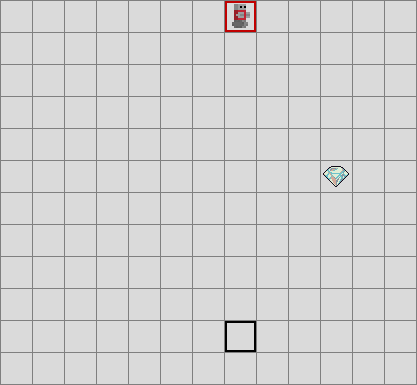
\includegraphics[width=\linewidth]{images/envs/lvl1.png}
        \caption{Level 1 for debugging purposes.\newline}
    \end{subfigure}
    \hfill
    \begin{subfigure}[t]{0.31\linewidth}
        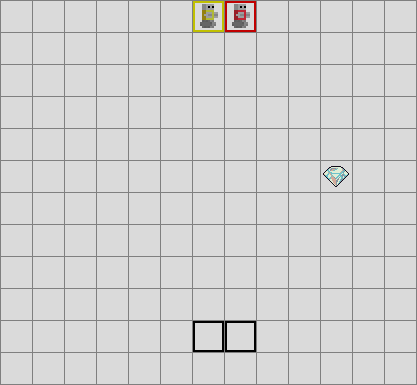
\includegraphics[width=\linewidth]{images/envs/lvl2.png}
        \caption{Level 2, first step into multi-agent problems, almost no interdependence.}
    \end{subfigure}
    \hfill
    \begin{subfigure}[t]{0.31\linewidth}
        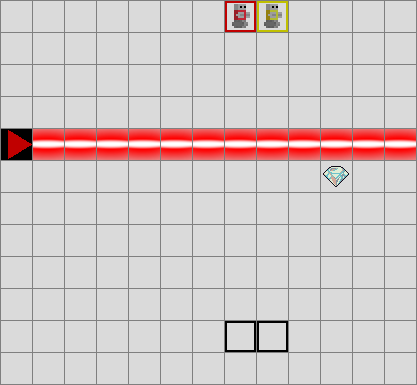
\includegraphics[width=\linewidth]{images/envs/lvl3.png}
        \caption{Level 3, introduces the dynamic of laser-blocking, which increases interdependence.}
    \end{subfigure}
    \begin{subfigure}[t]{0.31\linewidth}
        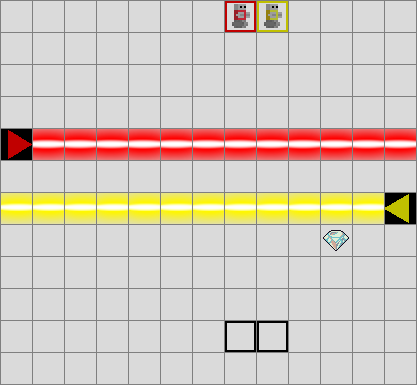
\includegraphics[width=\linewidth]{images/envs/lvl4.png}
        \caption{Level 4 introduces two lasers such that each agent successively has to block it for the other for even more interdependence.}
    \end{subfigure}
    \hfill
    \begin{subfigure}[t]{0.31\linewidth}
        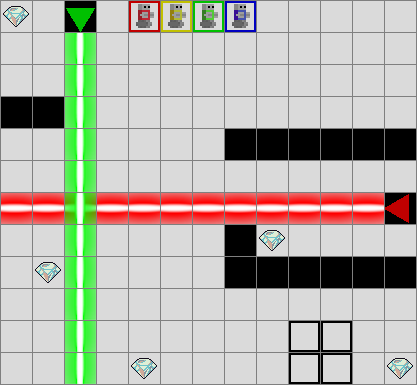
\includegraphics[width=\linewidth]{images/envs/lvl5.png}
        \caption{Level 5 also has 2 lasers but has 4 agents, which increases interdependence.}
    \end{subfigure}
    \hfill
    \begin{subfigure}[t]{0.31\linewidth}
        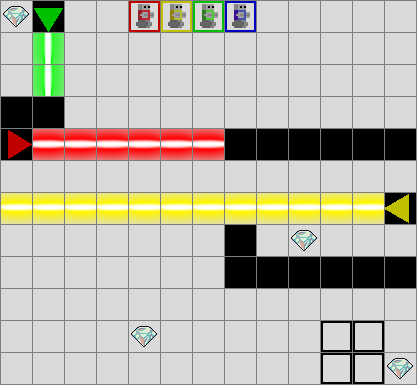
\includegraphics[width=\linewidth]{images/envs/lvl6.png}
        \caption{Level 6, four agents and three lasers, the most difficult level introduced with the highest level of interdependence.}
    \end{subfigure}
    \caption{Six standard levels of LLE. The levels have been designed with incremental level of interdependence in mind. Level 6 is the main level studied in this work.}
    \label{fig:my_label}
\end{figure}


\newpage
\section{Results on standard maps}
\label{apx:all-results}

\begin{figure}[h]
    \centering
    \begin{tikzpicture}
        \begin{groupplot}[
            group style={group size= 2 by 3},
            height=4.5cm,
            width=7cm, 
            grid=major,
            legend columns=2
            xtick={0, 200000, 400000, 600000, 800000, 1000000},
            xticklabels={0, 0, 200k, 400, 600k, 800k, 1m},
            scaled x ticks=false,
            title style={yshift=-0.2cm},
        ]
            \nextgroupplot[title={Level 1}, legend to name=mario, ymin=0, ymax=3.5, xmin=0, xmax=1000000]       
                \addplot[line width=1pt, mark=none, color=black, style=dashed] coordinates {(0,3) (1000000,3)};
                \addlegendentry{Max score}

                \plotLevelMean[IQL]{dqn}{lvl1};
                \plotLevelMean[VDN]{vdn}{lvl1};
                \plotLevelMean[QMix]{qmix}{lvl1};
            
                \plotLevelStd{dqn}{lvl1};
                \plotLevelStd{vdn}{lvl1};
                \plotLevelStd{qmix}{lvl1};

                \coordinate (top-left) at (rel axis cs:0,1);% coordinate at top left of the first plot
                \coordinate (bot-left) at (rel axis cs:0,0);
                
            \nextgroupplot[title={Level 2}, ymin=0, ymax=4.5, xmin=0, xmax=1000000]
                \addplot[line width=1pt, mark=none, color=black, style=dashed] coordinates {(0,4) (1000000,4)};
                \plotLevelMean{dqn}{lvl2};
                \plotLevelMean{vdn}{lvl2};
                \plotLevelMean{qmix}{lvl2};
                \addplot[black, samples=2] {0.5};
            
                \plotLevelStd{dqn}{lvl2};
                \plotLevelStd{vdn}{lvl2};
                \plotLevelStd{qmix}{lvl2};
                \coordinate (right) at (rel axis cs:1,1);
                \coordinate (bot) at (rel axis cs:1,0);% coordinate at bottom of the last plot

            \nextgroupplot[title={Level 3}, ymin=0, ymax=4.5, xmin=0, xmax=1000000]
                \addplot[line width=1pt, mark=none, color=black, style=dashed] coordinates {(0,4) (1000000,4)};
                \plotLevelMean{dqn}{lvl3};
                \plotLevelMean{vdn}{lvl3};
                \plotLevelMean{qmix}{lvl3};
            
                \plotLevelStd{dqn}{lvl3};
                \plotLevelStd{vdn}{lvl3};
                \plotLevelStd{qmix}{lvl3};

            \nextgroupplot[title={Level 4}, ymin=0, ymax=4.5, xmin=0, xmax=1000000]
                \addplot[line width=1pt, mark=none, color=black, style=dashed] coordinates {(0,4) (1000000,4)};
                \plotLevelMean{dqn}{lvl4};
                \plotLevelMean{vdn}{lvl4};
                \plotLevelMean{qmix}{lvl4};
            
                \plotLevelStd{dqn}{lvl4};
                \plotLevelStd{vdn}{lvl4};
                \plotLevelStd{qmix}{lvl4};

            \nextgroupplot[title={Level 5}, ymin=0, ymax=10.5, xmin=0, xmax=1000000]
                \addplot[line width=1pt, mark=none, color=black, style=dashed] coordinates {(0,10) (1000000,10)};
                \plotLevelMean{dqn}{lvl5};
                \plotLevelMean{vdn}{lvl5};
                \plotLevelMean{qmix}{lvl5};
            
                \plotLevelStd{dqn}{lvl5};
                \plotLevelStd{vdn}{lvl5};
                \plotLevelStd{qmix}{lvl5};

            \nextgroupplot[title={Level 6}, ymin=-1.15, ymax=9.5, xmin=0, xmax=1000000]
                \addplot[line width=1pt, mark=none, color=black, style=dashed] coordinates {(0,9) (1000000,9)};
                \plotMean{dqn}{score};
                \plotMean{vdn}{score};
                \plotMean{qmix}{score};
            
                \plotStd{dqn}{score};
                \plotStd{vdn}{score};            
                \plotStd{qmix}{score};

                
        \end{groupplot}
        \path (top-left)--(bot) coordinate[midway] (center);
        \path (top-left)--(bot-left) coordinate[midway] (center-left);
        \path (top-left)--(right) coordinate[midway] (h-center);
        \node[above=0.2cm, inner sep=0pt] at (h-center) {\pgfplotslegendfromname{mario}};
    \end{tikzpicture}
    \caption{Scores on standard maps over training time. Maximum score achievable is shown as a black dotted line. These results show the mean in bold $\pm$ the standard deviation, capped by minimum and maximum.}
\end{figure}




